\documentclass[a4paper,10pt]{report}
\usepackage{graphicx}
\usepackage[polish]{babel}
\usepackage[utf8]{inputenc}
\usepackage{polski}
\usepackage[T1]{fontenc}
\usepackage{indentfirst}
\usepackage{amsmath}
\usepackage{verbatim}
\usepackage{booktabs}
\usepackage{color}
\usepackage[usenames,dvipsnames,svgnames]{xcolor}
\usepackage{geometry}
\geometry{verbose,lmargin=3cm,rmargin=3cm}
\usepackage{utopia}
\frenchspacing

%opening
\title{Rozpoznawanie relacji sematycznych w tekscie, porzez klasyfikację kontekstu relacji przy pomocy klasyfikatora \textbf{CRF}}
\author{Jakub A. Gramsz \\ Michał Krautforst}
\date{24 stycznia 2014}

\begin{document}
\renewcommand{\figurename}{Wykres}
\renewcommand{\chaptername}{}

\maketitle
\tableofcontents

\chapter{Wstęp} % jest to wersja robocza

\section{Klasyfikator CRF} 

\subsection{Motywacja}

Klasyfikator CRF utworzony został pod kątem segmentacji i znakowania danych sekwencyjnych \cite{lafferty2001crf}. Klasyfikator ten często wykorzystywany w przetwarzaniu języka naturalnego, jest stosunkowo młodą metodą klasyfikacji, wykazująca potencjał do badań. Klasyfikator ten osiągną wysoką jakością klasyfikacji przy oznaczaniu nazw własnych w tekstach.

\subsection{Charakterystyka klasyfikatora}

Klasyfikator CRF został zaporoponowany aby przetwarzać sekwencje w obu kierunkach \cite{lafferty2001crf}.

\section{Rozpoznanie literatury}

\subsection{``Conditional random fields: Probabilistic models for segmenting and labeling sequence data'' \cite{lafferty2001crf}}

Artykuł w którym zaproponowano nowy klasyfikator (ang. Conditional random fields) służący do segmentacji lub etykietowania danych sekwencyjnych mający w tych zadaniach pokonywać wady ukrytych łańcuchów Markowa i gramatyk stochastycznych. Prezentowany klasyfikator przedstawiany jest również jako rozwiazanie ograniczeń modelów Markowa maksymalizujących entropię (MEMM) oraz innych modeli tego typu bazujących na grafach skierowanych. W artykule dokonano porównania efektywności oraz jakości etykietowania danych sekwencyjnych za pomocą CRF oraz HMM i MEMM. Wskazuje on na dużo lepsze wyniki uzyskane przez prezentowaną metodę CRF. 

\subsection{``Conditional random fields: An introduction'' \cite{wallach2004crf}}

Aktykuł opisujący działanie klasyfikatora CRF.

\subsection{``Document Summarization Using Conditional Random Fields'' \cite{shen2007doccum}}

Aktykuł opisujący wykożystanie CRF do zadania strzeszczania dokumentów.
Opisuje zastosowanie klasyfikatora do problemu z dziedziny Inżynierii Języka Naturalnego, wskazując mi. cechy wykorzystane do opisania danych.  

\subsection{``Integrating probabilistic extraction models and data mining to discover relations and patterns in text'' \cite{culotta2006integrating}}

Przedstawienie zadania odnajdywania relacji w tekście jako problem etykietowania danych sekwencyjnych z wykorzytsaniem CRF.


\chapter{Praca badawcza}

\section{Implementacja}

\noindent Poniżej przedstawiamy zadania.
\begin{enumerate}
 \item Wydobycie par hiponim-hiperonim o zadanej odległości między sobą wprost z bazy Słowosieci. % skryp to wyciągania par hiponim-hiperonim dla zadanej odległości
 \item Budowa grafu relacji hiperonimi. % graf relacji hiperonimi (działa za wolno)
 \item Oznaczenie otrzymanych par w zadanym korupusie. % skrypt oznaczający wyciągnięte pary w zadanym korpusie
 \item Podział korpusu na zbiór uczący oraz testujący. % skrypt dzielacy oznaczony korpus na dane uczace i testujace
 \item Wydobycie oznaczonych kontekstow. % skrypt co wyciagania oznaczonych kontekstow
 \item Wypisywanie przykładów false positive skrypt wypisujacy przyklady false positive.
 \item Dobór cech dla klasyfikatora \textbf{CRF}.  % badanie wpływu doboru cech
 \item Wyznacznanie odległości pomiędzy parami oznaczonymi poprzez klasyfikator (pośrednio oznaczonymi poprzez kontekst).  % skyrp do sprawdzania odległości wyodrębionych par
\end{enumerate}

\section{Badania}

\subsection{Zbiór uczący}

Zbiór uczący stanowią zdania pochodzące z korpusów języka polskiego z oznaczonymi kontekstami par słów znajdujących się w relacji hiperonimi znajdujących się w różnych odległościach od siebie (1 do 3) w słowosieci. Każdy token opisany wektorem cech.

\begin{itemize}
 \item korpus wykorzystany w testach - Korpus Języka Polskiego Politechniki Wrocławskiej
 \item długości kontekstów 5, 10, 15
 \item pary hiponim-hiperonim o odległościach 1, 2, 3.
\end{itemize}

\chapter{Wyniki i wnioski}

\section{Wyniki}

\begin{table}[htp]
  \centering
    \begin{tabular}{rrrrr}
    \toprule
    \multicolumn{1}{c}{kontekst} & \multicolumn{1}{c}{Odl. par} & \multicolumn{1}{c}{Precyzja} & \multicolumn{1}{c}{Kompletność} & \multicolumn{1}{c}{F-score} \\
    \midrule
    5     & 1     & 72.73\% & 18.18\% & 29.09\% \\
    15    & 1     & 69.57\% & 17.02\% & 27.35\% \\
    5     & 2     & 78.57\% & 14.86\% & 25.00\% \\
    10    & 2     & 70.83\% & 15.18\% & 25.00\% \\
    10    & 3     & 63.89\% & 15.44\% & 24.86\% \\
    5     & 3     & 80.00\% & 13.79\% & 23.53\% \\
    10    & 1     & 73.33\% & 13.25\% & 22.45\% \\
    15    & 2     & 48.65\% & 13.24\% & 20.81\% \\
    15    & 3     & 34.38\% & 7.10\% & 11.76\% \\
    \bottomrule
    \end{tabular}%
    \caption{Podsumowanie najlepszych wyników z badań jakości klasyfikatora względem długości kontekstu oraz odległości między leksemami w sensie relacji hiperonimi.}
  \label{tab:wyniki-podsum}%
\end{table}%

\begin{table}[htp]
  \centering
    \begin{tabular}{rrrrrrrrr}
    \toprule
    \multicolumn{1}{c}{Dł. Kontekstu} & \multicolumn{1}{c}{Odl. Par} & \multicolumn{1}{c}{Walidacja} & TP    & FP    & FN    & \multicolumn{1}{c}{Precyzja} & \multicolumn{1}{c}{Kompletność} & \multicolumn{1}{c}{F-score} \\
    \midrule
    5     & 1     & 7     & 25    & 3     & 110   & 89.29\% & 18.52\% & 30.67\% \\
    5     & 1     & 10    & 8     & 3     & 36    & 72.73\% & 18.18\% & 29.09\% \\
    15    & 1     & 10    & 16    & 7     & 78    & 69.57\% & 17.02\% & 27.35\% \\
    10    & 2     & 10    & 17    & 7     & 95    & 70.83\% & 15.18\% & 25.00\% \\
    5     & 2     & 10    & 11    & 3     & 63    & 78.57\% & 14.86\% & 25.00\% \\
    10    & 3     & 10    & 23    & 13    & 126   & 63.89\% & 15.44\% & 24.86\% \\
    5     & 1     & 5     & 33    & 0     & 202   & 100.00\% & 14.04\% & 24.63\% \\
    5     & 2     & 5     & 51    & 10    & 313   & 83.61\% & 14.01\% & 24.00\% \\
    5     & 2     & 7     & 31    & 15    & 186   & 67.39\% & 14.29\% & 23.57\% \\
    5     & 3     & 10    & 12    & 3     & 75    & 80.00\% & 13.79\% & 23.53\% \\
    10    & 3     & 7     & 61    & 34    & 370   & 64.21\% & 14.15\% & 23.19\% \\
    5     & 3     & 5     & 60    & 17    & 389   & 77.92\% & 13.36\% & 22.81\% \\
    5     & 3     & 7     & 37    & 13    & 239   & 74.00\% & 13.41\% & 22.70\% \\
    10    & 1     & 10    & 11    & 4     & 72    & 73.33\% & 13.25\% & 22.45\% \\
    10    & 2     & 7     & 48    & 28    & 309   & 63.16\% & 13.45\% & 22.17\% \\
    15    & 2     & 10    & 18    & 19    & 118   & 48.65\% & 13.24\% & 20.81\% \\
    15    & 1     & 7     & 35    & 20    & 262   & 63.64\% & 11.78\% & 19.89\% \\
    10    & 1     & 7     & 24    & 12    & 224   & 66.67\% & 9.68\% & 16.90\% \\
    10    & 3     & 5     & 70    & 73    & 671   & 48.95\% & 9.45\% & 15.84\% \\
    10    & 1     & 5     & 34    & 13    & 366   & 72.34\% & 8.50\% & 15.21\% \\
    15    & 1     & 5     & 42    & 25    & 446   & 62.69\% & 8.61\% & 15.14\% \\
    15    & 3     & 7     & 43    & 69    & 425   & 38.39\% & 9.19\% & 14.83\% \\
    15    & 2     & 7     & 32    & 38    & 358   & 45.71\% & 8.21\% & 13.91\% \\
    15    & 3     & 5     & 58    & 103   & 726   & 36.02\% & 7.40\% & 12.28\% \\
    15    & 3     & 10    & 11    & 21    & 144   & 34.38\% & 7.10\% & 11.76\% \\
    15    & 2     & 5     & 36    & 58    & 639   & 38.30\% & 5.33\% & 9.36\% \\
    \bottomrule
    \end{tabular}%
    \caption{Wszystkie wyniki otrzymane w wyniku badań jakości klasyfikatora względem długości kontekstu oraz odległości między leksemami w sensie relacji hiperonimi.}
  \label{tab:addlabel}%
\end{table}%


% \begin{table}[htp]
%   \centering
% 
%     \begin{tabular}{rrrrr}
%     \toprule
%     \multicolumn{1}{c}{kontekst} & \multicolumn{1}{c}{odl. par} & \multicolumn{1}{c}{Precyzja} & \multicolumn{1}{c}{Kompletność} & \multicolumn{1}{c}{F-score} \\
%     \midrule
%     1     & 7     & 89.29\% & 18.52\% & 30.67\% \\
%     1     & 10    & 72.73\% & 18.18\% & 29.09\% \\
%     1     & 10    & 69.57\% & 17.02\% & 27.35\% \\
%     2     & 10    & 78.57\% & 14.86\% & 25.00\% \\
%     2     & 10    & 70.83\% & 15.18\% & 25.00\% \\
%     3     & 10    & 63.89\% & 15.44\% & 24.86\% \\
%     1     & 5     & 100.00\% & 14.04\% & 24.63\% \\
%     2     & 5     & 83.61\% & 14.01\% & 24.00\% \\
%     2     & 7     & 67.39\% & 14.29\% & 23.57\% \\
%     3     & 10    & 80.00\% & 13.79\% & 23.53\% \\
%     3     & 7     & 64.21\% & 14.15\% & 23.19\% \\
%     3     & 5     & 77.92\% & 13.36\% & 22.81\% \\
%     3     & 7     & 74.00\% & 13.41\% & 22.70\% \\
%     1     & 10    & 73.33\% & 13.25\% & 22.45\% \\
%     2     & 7     & 63.16\% & 13.45\% & 22.17\% \\
%     2     & 10    & 48.65\% & 13.24\% & 20.81\% \\
%     1     & 7     & 63.64\% & 11.78\% & 19.89\% \\
%     1     & 7     & 66.67\% & 9.68\% & 16.90\% \\
%     3     & 5     & 48.95\% & 9.45\% & 15.84\% \\
%     1     & 5     & 72.34\% & 8.50\% & 15.21\% \\
%     1     & 5     & 62.69\% & 8.61\% & 15.14\% \\
%     3     & 7     & 38.39\% & 9.19\% & 14.83\% \\
%     2     & 7     & 45.71\% & 8.21\% & 13.91\% \\
%     3     & 5     & 36.02\% & 7.40\% & 12.28\% \\
%     3     & 10    & 34.38\% & 7.10\% & 11.76\% \\
%     2     & 5     & 38.30\% & 5.33\% & 9.36\% \\
%     \bottomrule
%     \end{tabular}%
%   \caption{Add caption}
%   \label{tab:wyniki-wszy}%
% \end{table}%



\begin{figure}[h]
\centering
 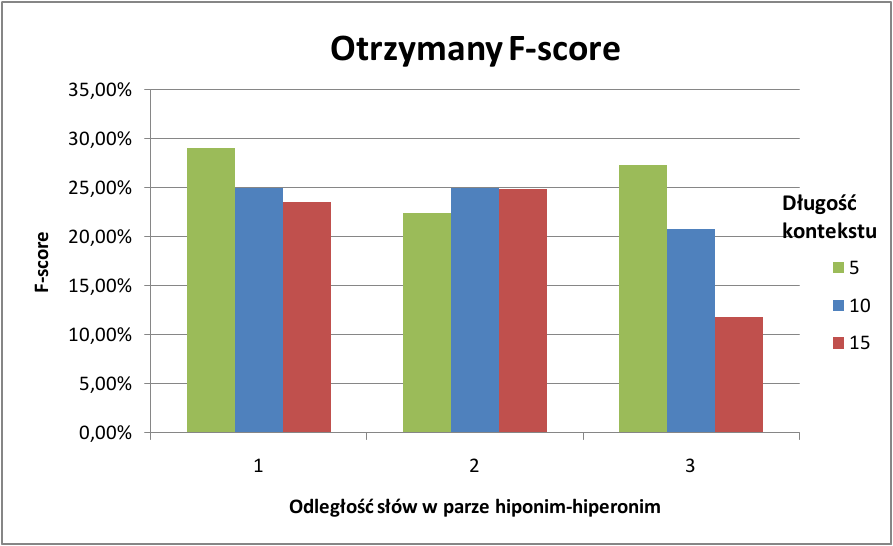
\includegraphics[width=13cm]{img/image001.png}
 \caption{Porównanie F-score klasyfikatorów w zależności od długości kontekstów oraz odległości pomiędzy hiponimem a hiperonimem w parach.}
\label{fig:wykres}
\end{figure} 

\section{Wnioski}


\begin{itemize}
\item Badania prowadzone były na stosunkowo małym korpusie, warto przeprowadzić analogiczne testy dla większej ilości danych,
napotkano jednak problem w postaci bardzo dużego zapotrzebowania na zasoby pamięci.  

\item Skorzystanie z par hiponim-hiperonim o większej odległości powoduje spadek precyzji bez zmian kompletności.

\item Długość kontekstu wpływa na liczbę wygenerowanych przykładów pozytywnych, jednak wraz z jego wzrostem spada jakość klasyfikacji.

\item Manipulacja cechami niezauważalnie wpływa na wyniki (cech powinno być możliwie dużo)

\item Zmniejszenie liczby negatywnych przypadków pogarsza jakość klasyfikacji. Należałoby zrównoważyć proporcje liczby przypadków pozytywnych i negatywnych, jednak trudne jest określenie kryterium.

\item Klasyfikacja cechuje się wysoką precyzją, mimo zróżnicowanych przypadków pozytywnych oraz rzadkiej powtarzalności kontekstów

\item Zaproponowana metoda odnajdowania relacji sematycznych w tekście poprzez oznaczanie ich kontekstów, nie przynosi zadowalających rezultatów, niemniej jednak może stanowić dobry wstęp na podstawie, którego innymi metodami można by proces ten kontynuować. Przykładowo oznaczone konteksty można by grupować na podstawie ich podobieństwa a następnie wyciągać z nich bardziej ogólne wzorce.

\end{itemize}

%Bibliografia
\bibliographystyle{abbrv}
\nocite{*}
\bibliography{sem-rel-crf}

\end{document}
